A lo largo de los capítulos anteriores modelamos el canal de transmisión simplemente como un sistema lineal e invariante en el tiempo, caracterizado por su respuesta en frecuencia $\hat{H}(f)$ (Figura \ref{fig:distorsion canal}), sin preguntarnos de dónde surgía dicha respuesta, ni por qué introducía atenuación, ancho de banda limitado o interferencia intersimbólica. En este capítulo le damos contenido físico a ese bloque gris, para el caso de un canal \emph{guiado}: un par de conductores paralelos, un par trenzado o un cable coaxial, que conducen la señal eléctrica de un extremo a otro. El objetivo es llegar, a partir de primeros principios, a la respuesta en frecuencia $\hat{H}(f)$ de un tramo de línea, que es exactamente el objeto que el resto de estas notas ya utiliza.

\section{Modelo de parámetros distribuidos}\label{sec:parametros distribuidos}

Cuando trabajamos con circuitos a bajas frecuencias, es habitual despreciar el tiempo que tardan las señales en propagarse dentro de los componentes: se supone que la tensión y la corriente son las mismas en todo punto de un cable, en cualquier instante. Esta aproximación de \emph{parámetros concentrados} es válida cuando la longitud física del circuito es mucho menor que la longitud de onda $\lambda = v/f$ de las señales involucradas, siendo $v$ la velocidad de propagación en el medio. En comunicaciones esto deja de ser cierto: a $f=100\ \unit{\mega\hertz}$, con una velocidad de propagación típica en un cable de $v\approx 2\times 10^8\ \unit{\meter\per\second}$, la longitud de onda es de apenas $\lambda = 2\ \unit{\meter}$, comparable o menor a la longitud de un cable de conexión típico. En este régimen ya no podemos ignorar el tiempo de tránsito de la señal a lo largo de la línea: la tensión y la corriente pasan a depender tanto del tiempo $t$ como de la posición $z$ a lo largo del cable. Este es el modelo de \emph{parámetros distribuidos} que desarrollamos a continuación.

La idea central es discretizar la línea en segmentos infinitesimales de longitud $\Delta z$ y modelar cada uno como un circuito de parámetros concentrados equivalente. Cuatro parámetros, definidos \emph{por unidad de longitud}, alcanzan para caracterizar el comportamiento eléctrico de la línea.

\begin{definicion}[Parámetros primarios de la línea]\label{def:parametros primarios}
Una línea de transmisión de dos conductores queda caracterizada por cuatro parámetros por unidad de longitud, en general dependientes de la frecuencia:
\begin{itemize}
    \item $R$ ($\unit{\ohm/\meter}$): resistencia serie de los conductores, debida a su conductividad finita.
    \item $L$ [$\unit{\henry}/\unit{\meter}$]: inductancia serie, asociada al campo magnético que rodea a los conductores cuando circula corriente por ellos.
    \item $G$ [$\unit{\siemens}/\unit{\meter}$]: conductancia paralelo, debida a las pérdidas (corrientes de fuga) en el dieléctrico que separa los conductores.
    \item $C$ [$\unit{\farad}/\unit{\meter}$]: capacidad paralelo, asociada al campo eléctrico entre los conductores.
\end{itemize}
\end{definicion}

Los cuatro parámetros dependen de la geometría de la línea (diámetro y separación de los conductores, material dieléctrico, etc.). Por ahora los tratamos como constantes conocidas, con la salvedad de que $R$ y $G$ dependen en realidad de la frecuencia; retomamos este punto con detalle en la Sección \ref{sec:dispersion pulsos}, donde esa dependencia resulta ser la causante de buena parte de la distorsión que sufren los pulsos.

Un segmento de línea de longitud $\Delta z$ se modela mediante el circuito de parámetros concentrados de la Figura \ref{fig:segmento linea}: una resistencia $R\Delta z$ en serie con una inductancia $L\Delta z$, seguida de una conductancia $G\Delta z$ en paralelo con una capacidad $C\Delta z$, ambas conectando el conductor de señal con el de retorno.

\begin{figure}
    \begin{center}
        \begin{circuitikz}[scale=1.5, american]
            \draw (0,0) to[R=$R\Delta z$] (1.9,0) to[L=$L\Delta z$] (4,0);
            \draw (4,0) -- (4.4,0);
            \draw (4,0) to[R=$1/G\Delta z$] (4,-1.1) to[C=$C\Delta z$] (4,-2.2);
            \draw (0,-2.2) -- (4,-2.2);
            \draw (4,-2.2) -- (4.4,-2.2);
            \draw[-latex, thick] (0,-1.85) -- (0,-0.35) node[midway,left] {$v(z,t)$};
            \draw[-latex, thick] (1.6,0.5) -- (2.4,0.5) node[midway,above] {$i(z,t)$};
            \node[below left] at (0,-2.2) {$z$};
            \node[below right] at (4.4,-2.2) {$z+\Delta z$};
        \end{circuitikz}
    \end{center}
    \caption{Circuito de parámetros concentrados equivalente a un segmento de línea de longitud $\Delta z$. La línea completa es la cascada de infinitos segmentos de este tipo.}\label{fig:segmento linea}
\end{figure}

\subsection*{Ecuaciones del telegrafista}

Apliquemos las leyes de Kirchhoff al segmento de la Figura \ref{fig:segmento linea}. Sean $v(z,t)$ e $i(z,t)$ la tensión y la corriente en la posición $z$ de la línea, en el instante $t$. Recorriendo la malla serie del segmento, la ley de tensiones de Kirchhoff da:
\begin{equation*}
    v(z,t) = R\Delta z\, i(z,t) + L\Delta z\, \frac{\partial i(z,t)}{\partial t} + v(z+\Delta z,t).
\end{equation*}
Reordenando y dividiendo entre $\Delta z$:
\begin{equation*}
    \frac{v(z+\Delta z,t) - v(z,t)}{\Delta z} = -R\, i(z,t) - L\, \frac{\partial i(z,t)}{\partial t}.
\end{equation*}
Tomando el límite $\Delta z \to 0$, el miembro izquierdo es por definición $\partial v(z,t)/\partial z$. De manera análoga, aplicando la ley de corrientes de Kirchhoff al nodo entre los dos segmentos (la corriente que ``se fuga'' hacia el retorno a través de $G\Delta z$ y $C\Delta z$ es $i(z,t)-i(z+\Delta z,t)$):
\begin{equation*}
    i(z,t) - i(z+\Delta z, t) = G\Delta z\, v(z+\Delta z,t) + C \Delta z\, \frac{\partial v(z+\Delta z,t)}{\partial t},
\end{equation*}
que en el mismo límite $\Delta z \to 0$ da $-\partial i(z,t)/\partial z$ en el miembro izquierdo. Se obtiene así el siguiente sistema de ecuaciones diferenciales en derivadas parciales, acopladas, conocidas como las \emph{ecuaciones del telegrafista}:
\begin{subequations}\label{eq:telegrafista}
\begin{align}
    \frac{\partial v(z,t)}{\partial z} &= -R\, i(z,t) - L\, \frac{\partial i(z,t)}{\partial t}, \\
    \nonumber \\ 
    \frac{\partial i(z,t)}{\partial z} &= -G\, v(z,t) - C\, \frac{\partial v(z,t)}{\partial t}.
\end{align}    
\end{subequations}
Estas ecuaciones, planteadas por Kelvin y luego completadas por Heaviside en el contexto del cable telegráfico transatlántico, son el punto de partida de todo el análisis de líneas de transmisión: relacionan cómo cambia la tensión en el espacio con cómo cambia la corriente en el tiempo y viceversa, acoplando así la dimensión espacial que el modelo de parámetros concentrados ignoraba.

\section{Ecuación de onda y propagación en la línea}\label{sec:ecuacion de onda}

Derivando la primera ecuación de \eqref{eq:telegrafista} respecto de $z$ y sustituyendo en la segunda, se obtiene una única ecuación de segundo orden para $v(z,t)$ (y, de forma simétrica, otra para $i(z,t)$):
\begin{equation}\label{eq:onda con perdidas}
    \frac{\partial^2 v(z,t)}{\partial z^2} = LC\, \frac{\partial^2 v(z,t)}{\partial t^2} + (RC+LG)\, \frac{\partial v(z,t)}{\partial t} + RG\, v(z,t).
\end{equation}

Esta ecuación se denomina \emph{ecuación de onda de la línea con pérdidas}. 

\begin{ejemplo}[Línea sin pérdidas]
    Supongamos un caso ideal de línea sin pérdidas, es decir $R=G=0$. En este caso la ecuación \eqref{eq:onda con perdidas} se reduce a:
    \begin{equation*}
        \frac{\partial^2 v}{\partial z^2} = LC\, \frac{\partial^2 v}{\partial t^2}.
    \end{equation*}
Esta es la ecuación de onda clásica, cuya solución general es $v(z,t) = f(t-z/v_0) + g(t+z/v_0)$ con $v_0=1/\sqrt{LC}$, denominada velocidad de propagación. Se trata entonces de dos formas de onda $f$ y $g$ genéricas viajando sin distorsión, una en cada sentido. 
\end{ejemplo}

Con pérdidas, sin embargo, esta ecuación no tiene en general una solución tan simple en el dominio temporal. Sin embargo, como el sistema \eqref{eq:telegrafista} es lineal e invariante en el tiempo (para $z$ fijo, $R,L,G,C$ no dependen de $t$), conviene resolverlo trabajando en frecuencia, tal como en la teoría general de sistemas LTI. Tomando transformada de Fourier en $t$ a ambos miembros de \eqref{eq:telegrafista}, definimos:
\begin{equation*}
v(z,t) \fourier \hat{V}(z,f), \quad \quad i(z,t) \fourier \hat{I}(z,f).
\end{equation*}
Usando que derivar en $t$ equivale a multiplicar por $j2\pi f$, se obtiene, para cada frecuencia $f$, un sistema de ecuaciones diferenciales \emph{ordinarias} en $z$:
\begin{equation}\label{eq:telegrafista fourier}
    \begin{aligned}
        \frac{d\hat{V}(z,f)}{dz} &= -\left(R+j2\pi f L\right)\hat{I}(z,f), \\
        \frac{d\hat{I}(z,f)}{dz} &= -\left(G+j2\pi f C\right)\hat{V}(z,f).
    \end{aligned}
\end{equation}
Derivando la primera ecuación respecto de $z$ y sustituyendo la segunda:
\begin{equation}\label{eq:onda perdida fourier}
    \frac{d^2\hat{V}(z,f)}{dz^2} = \left(R+j2\pi f L\right)\left(G+j2\pi f C\right) \hat{V}(z,f) = \gamma(f)^2\, \hat{V}(z,f),
\end{equation}
donde definimos la \emph{constante de propagación}:
\begin{equation}\label{eq:gamma}
    \gamma(f) := \alpha(f) + j\beta(f) = \sqrt{\left(R+j2\pi f L\right)\left(G+j2\pi f C\right)}.
\end{equation}

Notar que $\gamma(f)$ es en principio la raíz cuadrada de un número complejo: elegimos aquella raíz que posee $\alpha(f)\geqslant 0$. Esto corresponde a una elección física: las ondas se atenúan al propagarse (en la dirección $z$ creciente). De este modo, $\alpha(f)$ se denomina la \emph{constante de atenuación} y posee unidades de $\unit{\per\meter}$, aunque es común expresarla en $\unit{\deci\bel\per\meter}$. A $\beta(f)$ se le denomina \emph{constante de fase} y su unidad es $\unit{\radian/\meter}$.

La ecuación diferencial \eqref{eq:onda perdida fourier} es, para cada $f$, una ecuación de segundo orden en $z$ que posee como solución general:
\begin{equation}\label{eq:solucion V}
    \hat{V}(z,f) = \hat{V}^+(f)\, e^{-\gamma(f) z} + \hat{V}^-(f)\, e^{\gamma(f) z},
\end{equation}
donde las constantes $\hat{V}^+(f)$, $\hat{V}^-(f)$ precisamente pueden depender de $f$, así como de las condiciones de borde de la línea.

Interpretemos entonces cada uno de estos términos:
\begin{itemize}
    \item $\hat{V}^+(f)\, e^{-\gamma(f) z} = \hat{V}^+(f)e^{-\alpha(f) z}e^{-j\beta(f) z}$
\end{itemize}

el primer término, $\hat{V}^+(f)\e^{-\alpha(f) z}\e^{-j\beta(f) z}$, se atenúa a medida que $z$ crece y acumula un atraso de fase creciente con $z$: corresponde, al antitransformar, a una onda que se propaga en el sentido de $z$ creciente y llega retardada y atenuada -- la llamamos \emph{onda incidente}. El segundo término, con $\e^{+\gamma(f) z}$, crece con $z$: no es físico para una línea semi-infinita, pero si la línea tiene longitud finita y termina en una carga que refleja parte de la energía (Sección \ref{sec:linea cargada}), representa la \emph{onda reflejada}, que se propaga en el sentido de $z$ decreciente y por lo tanto se atenúa a medida que $z$ decrece.

Sustituyendo \eqref{eq:solucion V} en la primera ecuación de \eqref{eq:telegrafista fourier} se obtiene $\hat I(z,f)$:
\begin{equation*}
    \hat{I}(z,f) = \frac{\gamma(f)}{R+j2\pi f L}\left[\hat{V}^+(f)\, \e^{-\gamma(f) z} - \hat{V}^-(f)\, \e^{\gamma(f) z}\right] = \frac{1}{Z_0(f)}\left[\hat{V}^+(f)\, \e^{-\gamma(f) z} - \hat{V}^-(f)\, \e^{\gamma(f) z}\right],
\end{equation*}
donde definimos la \emph{impedancia característica} de la línea:
\begin{equation}\label{eq:Z0}
    Z_0(f) := \frac{R+j2\pi f L}{\gamma(f)} = \sqrt{\frac{R+j2\pi f L}{G+j2\pi f C}}.
\end{equation}
$Z_0(f)$ es la relación entre tensión y corriente de \emph{cada onda por separado} ($\hat V^+/\hat I^+ = Z_0$, y $\hat V^-/\hat I^- = -Z_0$, el signo por viajar en sentido contrario): es la impedancia que ``ve'' una onda viajera en una línea infinita, y depende únicamente de los parámetros primarios de la línea, no de su longitud ni de lo que haya conectado en los extremos. En general $Z_0(f)$ es compleja.

\begin{remark}[Casos particulares importantes]
Dos casos especiales de \eqref{eq:gamma}--\eqref{eq:Z0} van a aparecer repetidamente:
\begin{itemize}
    \item \emph{Línea sin pérdidas} ($R=G=0$, una idealización razonable para cables de buena calidad en un rango moderado de frecuencias): $\gamma(f)=j2\pi f\sqrt{LC}$ es puramente imaginaria ($\alpha=0$, no hay atenuación) y $Z_0=\sqrt{L/C}$ es real y constante, independiente de la frecuencia.
    \item \emph{Línea con pérdidas pequeñas} ($R\ll 2\pi f L$, $G \ll 2\pi f C$): es la situación típica en RF, y da lugar a las aproximaciones que usamos en la Sección \ref{sec:dispersion pulsos}.
\end{itemize}
\end{remark}

\subsection*{Velocidad de fase y velocidad de grupo}

De \eqref{eq:solucion V}, cada componente de frecuencia $f$ de la onda incidente acumula, al recorrer una distancia $z$, un atraso de fase $\beta(f) z$ radianes. Definimos la \emph{velocidad de fase}:
\begin{equation*}
    v_p(f) := \frac{2\pi f}{\beta(f)},
\end{equation*}
la velocidad a la que se desplaza un punto de fase constante (por ejemplo, un máximo) de la sinusoide de frecuencia $f$. Si transmitimos una señal de banda ancha -- como un pulso -- cada componente espectral viaja, en principio, a su propia $v_p(f)$. Lo que le interesa a un observador que sigue la \emph{envolvente} del pulso (el paquete de energía) es la \emph{velocidad de grupo}:
\begin{equation*}
    v_g(f) := \left.\left(\frac{d\beta}{d\omega}\right)^{-1}\right|_{\omega=2\pi f} = \left.\frac{2\pi}{d\beta/df}\right|_{f}.
\end{equation*}
Si $\beta(f)$ es exactamente lineal en $f$, ambas velocidades coinciden y son independientes de $f$: todas las componentes espectrales del pulso viajan juntas, sin desarmarse. Si $\beta(f)$ no es lineal, distintas componentes de frecuencia viajan a distinta velocidad de fase y el pulso se \emph{dispersa} -- se ensancha en el tiempo. Este es, adelantando lo que viene en la Sección \ref{sec:dispersion pulsos}, uno de los dos mecanismos físicos que originan la ISI de la Sección \ref{sec:interferencia intersimbolica}.

\begin{condicion}[Condición de Heaviside -- línea sin distorsión]\label{cond:heaviside}
Si los parámetros primarios de la línea satisfacen
\begin{equation*}
    \frac{R}{L} = \frac{G}{C},
\end{equation*}
entonces $\alpha(f)$ es constante (no depende de $f$) y $\beta(f)$ es exactamente lineal en $f$, por lo que $v_p(f)=v_g(f)$ es también constante. Además, $Z_0(f)$ resulta real y constante. Una línea que verifica esta condición transmite cualquier forma de onda sin distorsión de fase: la señal recibida es una copia atenuada y retardada de la transmitida.
\end{condicion}

\begin{proof}
Sea $k:=R/L=G/C$. Entonces $R+j2\pi f L = L(k+j2\pi f)$ y $G+j2\pi f C = C(k+j2\pi f)$, por lo que:
\begin{equation*}
    \gamma(f) = \sqrt{LC}\,(k+j2\pi f) = \underbrace{k\sqrt{LC}}_{\alpha,\ \text{constante}} + j\underbrace{2\pi f \sqrt{LC}}_{\beta(f),\ \text{lineal en } f},
\end{equation*}
de donde $v_p(f)=v_g(f)=1/\sqrt{LC}$, constante. Para $Z_0$:
\begin{equation*}
    Z_0(f) = \sqrt{\frac{L(k+j2\pi f)}{C(k+j2\pi f)}} = \sqrt{\frac{L}{C}},
\end{equation*}
real y constante, independiente de $f$.
\end{proof}

La Condición de Heaviside es, en la práctica, difícil de lograr exactamente (típicamente requeriría aumentar $G$ artificialmente, lo cual es indeseable porque incrementa las pérdidas), pero cumple un rol importante como \emph{caso de referencia ideal}: es la situación en la que un cable se comporta, para cualquier señal, como un simple atenuador con retardo -- sin ISI de origen físico en la línea. Las líneas reales no verifican esta condición, y es precisamente esa desviación la que estudiamos en la Sección \ref{sec:dispersion pulsos}.

\begin{ejemplo}[Parámetros típicos de un cable coaxil]\label{ejemplo:coaxil parametros}
Consideremos un cable coaxil con parámetros (de orden de magnitud típico para un coaxil de $50\ \Omega$) $L=250\ \unit{\nano\henry\per\meter}$, $C=100\ \unit{\pico\farad\per\meter}$, $R=0.1\ \Omega/\unit{\meter}$ y $G\approx 0$ (dieléctrico de muy baja pérdida). Notemos primero que, sin pérdidas, $Z_0=\sqrt{L/C}=\sqrt{250\times 10^{-9}/100\times 10^{-12}}=50\ \Omega$, el valor nominal esperado.

A $f=10\ \unit{\mega\hertz}$: $2\pi f L \approx 15.7\ \Omega/\unit{\meter}$, mucho mayor que $R=0.1\ \Omega/\unit{\meter}$, y $2\pi f C \approx 6.28\times 10^{-3}\ \unit{\siemens}/\unit{\meter}$, mucho mayor que $G\approx 0$: estamos en el régimen de pérdidas pequeñas. Calculando \eqref{eq:gamma} numéricamente:
\begin{equation*}
    \gamma(10\ \unit{\mega\hertz}) = \sqrt{(0.1+j15.7)(0+j6.28\times 10^{-3})} \approx 1.0\times 10^{-3} + j\, 0.314\ \unit{\per\meter},
\end{equation*}
es decir $\alpha \approx 1.0\times 10^{-3}\ \unit{\neper\per\meter} \approx 8.7\times 10^{-3}\ \unit{\deci\bel\per\meter}$ (que en $100\ \unit{\meter}$ da $0.87\ \unit{\deci\bel}$, una atenuación moderada), y $\beta\approx 0.314\ \unit{\radian\per\meter}$, de donde $v_p = 2\pi f/\beta \approx 2\times 10^8\ \unit{\meter\per\second}$, es decir, aproximadamente $\frac{2}{3}$ de la velocidad de la luz en el vacío -- un valor típico para el factor de velocidad de un cable coaxil real.
\end{ejemplo}

En la Sección \ref{sec:dispersion pulsos} retomamos este mismo cable, pero prestando atención a lo que sucede cuando $R$ y $G$ dejan de ser tratables como constantes y empiezan a crecer con la frecuencia -- que es, en definitiva, el origen físico de la limitación de ancho de banda del canal guiado.

\section{Línea cargada: reflexión y adaptación}\label{sec:linea cargada}

Hasta ahora trabajamos con una línea infinita, donde solo existe la onda incidente ($\hat V^-\equiv 0$, nada hay más adelante que pueda generar una onda de regreso). En la práctica toda línea tiene longitud finita $\ell$ y termina conectada a una carga de impedancia $Z_L(f)$ -- por ejemplo, la entrada del receptor. Vamos a ver que, salvo en un caso particular, la carga genera una \emph{onda reflejada} que viaja de regreso hacia el generador, con consecuencias muy concretas sobre la señal que se transmite.

Ubiquemos el generador en $z=0$ y la carga en $z=\ell$. La condición de borde en la carga es simplemente la ley de Ohm generalizada: la tensión y la corriente en $z=\ell$ deben verificar $\hat V(\ell,f) = Z_L(f)\, \hat I(\ell,f)$. Sustituyendo \eqref{eq:solucion V} y la expresión de $\hat I(z,f)$ de la Sección \ref{sec:ecuacion de onda}:
\begin{equation*}
    \hat{V}^+(f)\e^{-\gamma\ell} + \hat{V}^-(f)\e^{\gamma\ell} = Z_L(f)\left[\hat{V}^+(f)\e^{-\gamma\ell} - \hat{V}^-(f)\e^{\gamma\ell}\right]\Big/ Z_0(f)\cdot Z_0(f),
\end{equation*}
que reordenando da la relación entre la amplitud de la onda reflejada y la incidente, \emph{evaluadas en la carga}:
\begin{equation}\label{eq:gamma L}
    \Gamma_L(f) := \frac{\hat{V}^-(f)\e^{\gamma\ell}}{\hat{V}^+(f)\e^{-\gamma\ell}} = \frac{Z_L(f)-Z_0(f)}{Z_L(f)+Z_0(f)}.
\end{equation}
Llamamos a $\Gamma_L(f)$ el \emph{coeficiente de reflexión de carga}. Notemos el caso particular $Z_L=Z_0$: la carga es indistinguible, para la línea, de que ésta continuara infinitamente -- no hay onda reflejada ($\Gamma_L=0$). Decimos que la línea está \emph{adaptada}. En cualquier otro caso, $\Gamma_L\neq 0$ y aparece una onda reflejada.

Definimos, más generalmente, el coeficiente de reflexión en cualquier punto $z$ de la línea como el cociente entre onda reflejada e incidente evaluadas en ese punto, $\Gamma(z,f):=\hat V^-(f)\e^{\gamma z}/(\hat V^+(f)\e^{-\gamma z})$. Es más cómodo trabajar con la distancia a la carga, $d:=\ell - z$ (que crece hacia el generador). De \eqref{eq:gamma L}:
\begin{equation}\label{eq:gamma d}
    \Gamma(d,f) = \Gamma_L(f)\, \e^{-2\gamma(f) d},
\end{equation}
es decir, el coeficiente de reflexión visto a una distancia $d$ de la carga es el de la carga, atenuado y rotado en fase por el recorrido de ida y vuelta (de ahí el factor $2$) hasta ese punto.

\subsection*{Impedancia vista a distancia $d$ de la carga}

Un resultado central en la práctica es que \emph{la impedancia que ve el generador no es $Z_L$, sino la que resulta de ``transformar'' $Z_L$ a través del tramo de línea}. Definiendo $Z(d,f):=\hat V(d,f)/\hat I(d,f)$ (con el mismo abuso de notación, usando $d$ como argumento), y repitiendo el cálculo que llevó a \eqref{eq:gamma L} pero ahora despejando $Z(d,f)$ en términos de $\Gamma(d,f)=\Gamma_L\e^{-2\gamma d}$:
\begin{equation*}
    Z(d,f) = Z_0(f)\, \frac{1+\Gamma(d,f)}{1-\Gamma(d,f)}.
\end{equation*}
Sustituyendo \eqref{eq:gamma d} y \eqref{eq:gamma L}, y operando (multiplicando numerador y denominador por $\e^{\gamma d}$, agrupando en $\cosh$ y $\sinh$, ver detalle en el Apéndice), se llega a la \emph{fórmula de transformación de impedancia}:
\begin{equation}\label{eq:transformacion impedancia}
    Z(d,f) = Z_0(f)\, \frac{Z_L(f) + Z_0(f)\tanh\left(\gamma(f) d\right)}{Z_0(f) + Z_L(f)\tanh\left(\gamma(f) d\right)}.
\end{equation}
En el caso usual de línea de bajas pérdidas, $\gamma(f)\approx j\beta(f)$, y usando que $\tanh(j\beta d) = j\tan(\beta d)$, \eqref{eq:transformacion impedancia} se reduce a la forma más citada en la práctica:
\begin{equation}\label{eq:transformacion impedancia sin perdidas}
    Z(d,f) = Z_0(f)\, \frac{Z_L(f) + jZ_0(f)\tan(\beta(f) d)}{Z_0(f) + jZ_L(f)\tan(\beta(f) d)} \qquad (\text{línea sin pérdidas}).
\end{equation}
Esta fórmula es periódica en $d$ con período $\lambda/2$ (ya que $\tan(\beta d)$ lo es), lo que da lugar a una propiedad notable: \emph{una línea de longitud media longitud de onda repite, en su entrada, la impedancia de la carga}; y una línea de un cuarto de longitud de onda \emph{invierte} la carga: $Z(\lambda/4) = Z_0^2/Z_L$, un resultado que se usa mucho como transformador de impedancia (el ``transformador de cuarto de onda'').

\subsection*{Onda estacionaria y ROE}

Como consecuencia de la reflexión, la tensión a lo largo de la línea deja de ser una simple onda viajera y pasa a ser la superposición de la incidente y la reflejada. Para una línea de bajas pérdidas ($\alpha\approx 0$), $|\Gamma(d,f)|=|\Gamma_L(f)|$ no depende de $d$ (de \eqref{eq:gamma d}, con $\gamma\approx j\beta$ puramente imaginaria, $|\e^{-2j\beta d}|=1$): el módulo del coeficiente de reflexión es el mismo en todo punto de la línea, solo cambia su fase. La magnitud de la tensión total,
\begin{equation*}
    |\hat V(d,f)| = |\hat V^+(f)|\, \left|1+\Gamma(d,f)\right| = |\hat V^+(f)|\, \left|1+|\Gamma_L(f)|\,\e^{j\theta(d)}\right|,
\end{equation*}
con $\theta(d)=\angle\Gamma_L - 2\beta d$ barriendo todos los valores posibles a medida que $d$ varía, oscila entre un máximo $|\hat V^+|(1+|\Gamma_L|)$ (cuando $\theta(d)=0$, las dos ondas en fase) y un mínimo $|\hat V^+|(1-|\Gamma_L|)$ (cuando $\theta(d)=\pi$, en contrafase): un patrón de \emph{onda estacionaria} a lo largo de la línea. Definimos la \emph{Relación de Onda Estacionaria} como el cociente entre ambos:
\begin{equation}\label{eq:roe}
    \mathrm{ROE} := \frac{|\hat V|_{\max}}{|\hat V|_{\min}} = \frac{1+|\Gamma_L(f)|}{1-|\Gamma_L(f)|} \in [1,\infty).
\end{equation}

\begin{remark}[ROE = VSWR]
La sigla ROE (Relación de Onda Estacionaria) es la traducción directa de VSWR (\emph{Voltage Standing Wave Ratio}), y ambas se usan indistintamente en la bibliografía, datasheets e instrumental -- muchos equipos muestran ``VSWR'' en pantalla aunque el manual esté en español. Históricamente, el ROE se medía físicamente deslizando una sonda a lo largo de una \emph{línea ranurada} y registrando los máximos y mínimos de tensión, de ahí el nombre.
\end{remark}

Dos casos extremos: si la línea está adaptada ($\Gamma_L=0$), $\mathrm{ROE}=1$ -- no hay onda estacionaria, toda la potencia incidente llega a la carga. Si la carga es un circuito abierto o un cortocircuito ($\Gamma_L=\pm 1$, reflexión total), $\mathrm{ROE}\to\infty$. El ROE es, en la práctica, la magnitud que se mide directamente con un instrumento (un ``medidor de ROE'' o \emph{VSWR meter}) conectado en la línea, ya que no requiere acceso a la fase de $\Gamma_L$, solo a los extremos del patrón de tensión.

\subsection*{La Carta de Smith}

La relación \eqref{eq:gamma L} es una transformación (de Möbius) entre la impedancia de carga y el coeficiente de reflexión. Es conveniente normalizar las impedancias respecto de $Z_0$, definiendo $\zeta:=Z/Z_0$ (usamos $\zeta$, y no $z$, para no confundir con la posición a lo largo de la línea). En términos de $\zeta_L=Z_L/Z_0$:
\begin{equation}\label{eq:gamma normalizado}
    \Gamma_L = \frac{\zeta_L - 1}{\zeta_L + 1} \qquad\Longleftrightarrow\qquad \zeta_L = \frac{1+\Gamma_L}{1-\Gamma_L}.
\end{equation}
Como toda carga físicamente realizable (pasiva) tiene $\mathrm{Re}(Z_L)\geqslant 0$, la transformación \eqref{eq:gamma normalizado} lleva todo el semiplano derecho $\mathrm{Re}(\zeta)\geqslant 0$ al disco unitario $|\Gamma_L|\leqslant 1$ -- consistente con que $\mathrm{ROE}\geqslant 1$ siempre. Una propiedad notable de las transformaciones de Möbius es que llevan rectas y circunferencias en rectas o circunferencias. En particular (ver Apéndice para el cálculo completo), las rectas de \emph{resistencia normalizada constante} $\mathrm{Re}(\zeta)=r$ se transforman en circunferencias en el plano $\Gamma$, centradas en $\left(\frac{r}{r+1},0\right)$ y de radio $\frac{1}{r+1}$; y las rectas de \emph{reactancia normalizada constante} $\mathrm{Im}(\zeta)=x$ se transforman en arcos de circunferencia centrados en $\left(1,\frac{1}{x}\right)$ y de radio $\frac{1}{|x|}$.

La \emph{Carta de Smith} (Figura \ref{fig:carta smith}) es, precisamente, un gráfico polar del disco $|\Gamma|\leqslant 1$ con esta grilla de circunferencias de $r$ y $x$ constante superpuesta, que permite pasar de $\zeta_L$ a $\Gamma_L$ y viceversa gráficamente, sin calcular \eqref{eq:gamma normalizado} a mano. Su verdadero valor práctico, sin embargo, está en lo que sucede al recorrer la línea: de \eqref{eq:gamma d}, moverse una distancia $d$ hacia el generador equivale, en el plano $\Gamma$, a \textbf{rotar} un ángulo $2\beta d$ (en sentido horario, alejándose de la carga) manteniendo el módulo $|\Gamma_L|$ constante -- es decir, \emph{moverse sobre una circunferencia centrada en el origen}. Y esa misma circunferencia, por \eqref{eq:roe}, es una curva de \textbf{ROE constante}. Encontrar $Z(d)$ para cualquier $d$ se reduce entonces a girar sobre un compás (la circunferencia de ROE constante que pasa por $\zeta_L$) el ángulo correspondiente y leer la impedancia normalizada en la grilla -- sin evaluar la tangente compleja de \eqref{eq:transformacion impedancia sin perdidas}.

\begin{figure}
    \begin{center}
        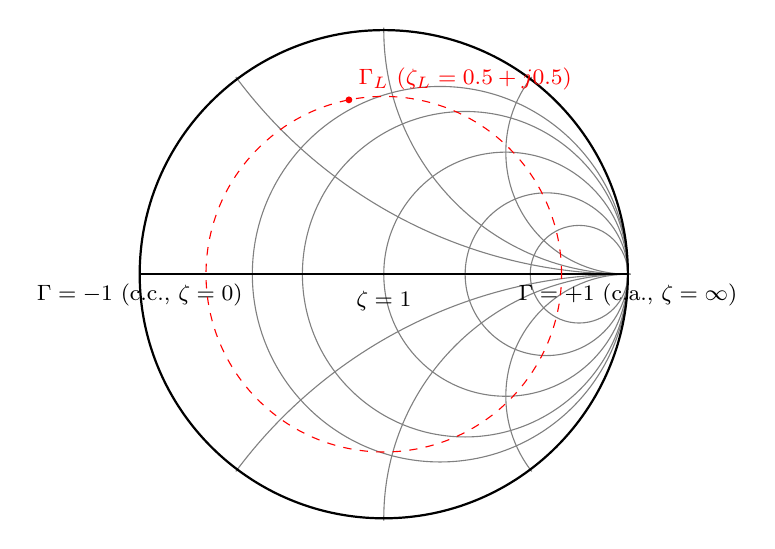
\begin{tikzpicture}[scale=3.1]
            \begin{scope}
                \clip (0,0) circle (1.01);
                \foreach \r in {0.3,0.5,1,2,4}{
                    \draw[thin, gray] ({\r/(\r+1)},0) circle ({1/(\r+1)});
                }
                \foreach \x in {0.5,1,2}{
                    \draw[thin, gray] (1,{1/\x}) circle ({1/\x});
                    \draw[thin, gray] (1,{-1/\x}) circle ({1/\x});
                }
            \end{scope}
            \draw[thick] (0,0) circle (1);
            \draw[thick] (-1,0) -- (1,0);
            \node[below] at (-1,0) {\footnotesize $\Gamma=-1$ (c.c., $\zeta=0$)};
            \node[below] at (1,0) {\footnotesize $\Gamma=+1$ (c.a., $\zeta=\infty$)};
            \node[below] at (0,-0.03) {\footnotesize $\zeta=1$};
            % ejemplo: zeta_L = 0.5 + j0.5 (coincide con ejemplo del texto: Z_L=25+j25 sobre Z0=50)
            \coordinate (GammaL) at ({(-0.2)/1.4}, {1/1.4});
            \fill[Red] (GammaL) circle (0.014);
            \node[Red, above right] at (GammaL) {\footnotesize $\Gamma_L$ ($\zeta_L=0.5+j0.5$)};
            \draw[Red, dashed] (0,0) circle ({sqrt(pow((-0.2)/1.4,2)+pow(1/1.4,2))});
        \end{tikzpicture}
    \end{center}
    \caption{Esquema de la Carta de Smith: disco $|\Gamma|\leqslant 1$ con la grilla de resistencia normalizada $r$ constante (circunferencias tangentes al punto $\Gamma=1$) y reactancia normalizada $x$ constante (arcos). Moverse a lo largo de la línea es rotar sobre la circunferencia punteada (ROE constante) que pasa por $\Gamma_L$.}\label{fig:carta smith}
\end{figure}

\begin{ejemplo}[Uso de la Carta de Smith]\label{ejemplo:smith}
Sobre una línea de $Z_0=50\ \Omega$ sin pérdidas se conecta una carga $Z_L=25+j25\ \Omega$, es decir $\zeta_L=0.5+j0.5$. Analíticamente, de \eqref{eq:gamma normalizado}:
\begin{equation*}
    \Gamma_L = \frac{(0.5+j0.5)-1}{(0.5+j0.5)+1} = \frac{-0.5+j0.5}{1.5+j0.5} = -0.2+j0.4,
\end{equation*}
de donde $|\Gamma_L|\approx 0.447$ y, por \eqref{eq:roe}, $\mathrm{ROE}=\frac{1+0.447}{1-0.447}\approx 2.62$. Sobre la Carta de Smith (Figura \ref{fig:carta smith}), el punto $\zeta_L=0.5+j0.5$ se ubica en la intersección de la circunferencia $r=0.5$ con el arco $x=0.5$, y se lee directamente $\Gamma_L$ como el vector desde el origen hasta ese punto -- sin necesidad de la cuenta algebraica anterior. La circunferencia de ROE constante que pasa por ese punto (marcada en la figura) es el lugar geométrico de todas las impedancias que se ven al recorrer la línea desde la carga: para hallar, por ejemplo, la impedancia a $d=\lambda/8$ del generador basta rotar $2\beta d = 2\cdot\frac{2\pi}{\lambda}\cdot\frac{\lambda}{8}=\frac{\pi}{2}$ ($90^\circ$) sobre esa circunferencia y leer $\zeta(d)$ en la grilla.
\end{ejemplo}

\subsection*{Adaptación de impedancias}

Un ROE alto no es solo un número: significa que buena parte de la potencia incidente no llega a la carga, sino que vuelve hacia el generador. En el mejor de los casos esto es ineficiente; en el peor, la onda reflejada puede dañar la fuente (por ejemplo, un amplificador de potencia mal protegido). Además, como veremos en la Sección \ref{sec:dispersion pulsos}, en una línea con pérdidas no despreciables un ROE alto empeora la atenuación efectiva total. Por todo esto, es habitual diseñar una red de \emph{adaptación} entre la línea y la carga, de manera que el generador vea $Z_0$ y $\Gamma=0$.

\paragraph{Transformador de cuarto de onda.} Cuando la carga es puramente resistiva, $Z_L=R_L$ (real), la Ecuación \eqref{eq:transformacion impedancia sin perdidas} ya nos da la herramienta: intercalando un tramo de longitud $\lambda/4$ de una línea auxiliar de impedancia característica
\begin{equation*}
    Z_0' = \sqrt{Z_0\, R_L},
\end{equation*}
la impedancia vista desde el generador es $Z_0'^2/R_L = Z_0$: adaptada. Este es, históricamente, el método usado para conectar una antena de $300\ \Omega$ (un dipolo doblado, alimentado por línea plana de dos conductores o \emph{twin-lead}, común en la recepción de TV analógica) a un cable coaxial estándar de $75\ \Omega$: se intercala un tramo de $\lambda/4$ de impedancia $Z_0'=\sqrt{75\cdot 300}=150\ \Omega$. El método es simple pero tiene una limitación importante: solo sirve para cargas reales, y además es angosto en banda (la condición $Z(\lambda/4)=Z_0'^2/Z_L$ solo vale exactamente a la frecuencia para la cual el tramo mide $\lambda/4$).

\paragraph{Adaptación con stub en paralelo.} Para una carga con parte reactiva, $Z_L=R_L+jX_L$, hace falta una técnica más general. La más común es el \emph{stub} (cabo) en paralelo: un tramo adicional de línea, del mismo $Z_0$, conectado en paralelo con la línea principal a una distancia $d$ de la carga, y terminado en circuito abierto o cortocircuito en su extremo libre. Como una línea sin pérdidas terminada en una reactancia pura ($Z_L=0$ o $Z_L=\infty$) presenta, en su entrada, una impedancia puramente reactiva (no disipa potencia), el stub actúa como un elemento reactivo variable, cuyo valor se ajusta con su longitud.

De \eqref{eq:transformacion impedancia sin perdidas}, tomando $Z_L=0$ (cortocircuito) se obtiene la impedancia de entrada de un stub cortocircuitado de longitud $\ell$: $Z_{cc}(\ell) = jZ_0\tan(\beta \ell)$; y tomando el límite $Z_L\to\infty$ (circuito abierto), $Z_{ca}(\ell) = -jZ_0\cot(\beta\ell)$. En admitancia normalizada ($y:=Y/Y_0$, $Y_0=1/Z_0$):
\begin{equation}\label{eq:stub susceptancias}
    y_{cc}(\ell) = -j\cot(\beta \ell), \qquad\qquad y_{ca}(\ell) = j\tan(\beta \ell),
\end{equation}
cada una capaz de sintetizar \emph{cualquier} susceptancia normalizada real con solo variar $\ell$ entre $0$ y $\lambda/2$. En la práctica se prefiere el stub cortocircuitado: el circuito abierto radia un poco por el extremo y es más sensible a efectos de borde, mientras que el cortocircuito es mecánicamente robusto y bien definido.

El procedimiento de adaptación con un stub en paralelo tiene dos pasos, y ambos se resuelven directamente sobre la Carta de Smith:
\begin{enumerate}
    \item \textbf{Buscar $d$:} avanzar desde la carga hacia el generador (rotando sobre la circunferencia de ROE constante que pasa por $\zeta_L$) hasta encontrar el punto donde la parte real de la admitancia normalizada vale $1$, es decir $y(d) = 1+jb$. Como trabajamos en paralelo, conviene pensar directamente en admitancias: por la simetría de \eqref{eq:gamma normalizado}, la admitancia normalizada correspondiente a un punto $\Gamma$ es exactamente la impedancia normalizada que se lee en la grilla en el punto \emph{diametralmente opuesto}, $-\Gamma$ -- mismo módulo, mismo círculo de ROE, rotado $180^\circ$. Esto permite usar la misma Carta de Smith de impedancias para leer admitancias, sin necesitar una grilla nueva.
    \item \textbf{Buscar $\ell$:} elegir la longitud del stub que cancela la parte imaginaria $b$ encontrada en el paso anterior, es decir tal que $y_{cc}(\ell) = -jb$ (usando \eqref{eq:stub susceptancias}). Con esto, la admitancia total en el punto de conexión es $1+jb-jb=1$: adaptado.
\end{enumerate}

\begin{ejemplo}[Adaptación con stub, continuación del Ejemplo \ref{ejemplo:smith}]
Retomemos la carga $\zeta_L=0.5+j0.5$ ($\Gamma_L=-0.2+j0.4$) del Ejemplo \ref{ejemplo:smith}. Su admitancia normalizada es:
\begin{equation*}
    y_L = \frac{1}{\zeta_L} = \frac{1}{0.5+j0.5} = 1-j1,
\end{equation*}
que en este caso particular ya tiene parte real $1$: la carga está, casualmente, exactamente sobre la circunferencia $g=1$ (sobre la Carta de Smith, esto se ve tomando el punto diametralmente opuesto a $\Gamma_L$, mismo círculo de ROE de la Figura \ref{fig:carta smith}). Esto simplifica el ejemplo: alcanza con un stub colocado \emph{en la carga misma}, $d=0$, así que solo resta el paso 2. Necesitamos cancelar $b=-1$, es decir un stub con $y_{cc}(\ell)=+j1 \Leftrightarrow -\cot(\beta\ell)=1 \Leftrightarrow \beta\ell = \frac{3\pi}{4}$, de donde:
\begin{equation*}
    \ell = \frac{3}{4}\cdot\frac{\pi}{\beta} = \frac{3}{4}\cdot\frac{\lambda}{2} = \frac{3\lambda}{8}.
\end{equation*}
Un stub cortocircuitado de longitud $\frac{3\lambda}{8}$, conectado en paralelo con la línea exactamente en la carga, adapta completamente este caso. En general (cuando $g_L\neq 1$) hace falta además el paso 1, buscando el $d\neq 0$ adecuado antes de calcular el largo del stub.
\end{ejemplo}

\section{Dispersión y su efecto sobre los pulsos}\label{sec:dispersion pulsos}

Ya tenemos todas las piezas para responder la pregunta que abrió este capítulo: ¿de dónde sale la respuesta en frecuencia $\hat H(f)$ que el resto de estas notas atribuye, sin más justificación, al canal (Figura \ref{fig:distorsion canal})? Consideremos una línea de longitud $\ell$ \emph{adaptada} en la carga ($Z_L=Z_0$, $\Gamma_L=0$, la situación deseable, que además evita las complicaciones de reflexión de la Sección \ref{sec:linea cargada}). En ese caso no hay onda reflejada, $\hat V(z,f)=\hat V^+(f)\,\e^{-\gamma(f) z}$ para todo $z$, y la tensión en la carga es simplemente la tensión de entrada, retardada y filtrada por el tramo de línea:
\begin{equation*}
    \hat V(\ell,f) = \hat V(0,f)\, \e^{-\gamma(f)\ell}.
\end{equation*}
Es decir, la línea se comporta exactamente como veníamos suponiendo desde el Capítulo \ref{chapter:modulacion banda base}: un sistema LTI, de respuesta en frecuencia
\begin{equation}\label{eq:H canal}
    \hat H(f) := \frac{\hat V(\ell,f)}{\hat V(0,f)} = \e^{-\gamma(f)\ell} = \underbrace{\e^{-\alpha(f)\ell}}_{\text{módulo}}\;\underbrace{\e^{-j\beta(f)\ell}}_{\text{fase}}.
\end{equation}
Esta es, en definitiva, la ecuación central del capítulo: le da contenido físico al bloque gris de la Figura \ref{fig:distorsion canal}. Si la línea verificara la Condición de Heaviside (Condición \ref{cond:heaviside}) -- $\alpha(f)$ constante y $\beta(f)$ exactamente lineal en $f$ -- \eqref{eq:H canal} sería, salvo una atenuación y un retardo constantes (ninguno de los dos un problema real para la detección: el primero se compensa con ganancia, el segundo con el instante de muestreo), un filtro ``todo pasa'': no distorsionaría la \emph{forma} de ningún pulso. La ISI de la Sección \ref{sec:interferencia intersimbolica} aparece precisamente porque las líneas reales \emph{no} verifican esa condición: tanto $\alpha(f)$ como $\beta(f)$ se apartan del caso ideal, por dos mecanismos físicos distintos, que estudiamos por separado antes de combinarlos.

\subsection*{Distorsión de fase}

El primer mecanismo es el que motivó la Condición de Heaviside: si $\beta(f)$ no es exactamente lineal en $f$, distintas componentes espectrales del pulso viajan a distinta velocidad de fase y, más precisamente, a distinta \emph{velocidad de grupo} $v_g(f)$ (Sección \ref{sec:ecuacion de onda}). El tiempo que tarda cada componente de frecuencia $f$ en atravesar la línea es el \emph{retardo de grupo}:
\begin{equation*}
    \tau_g(f) := \frac{\ell}{v_g(f)} = \ell\left.\frac{d\beta}{d\omega}\right|_{\omega=2\pi f}.
\end{equation*}
Si $\tau_g(f)$ es constante dentro del ancho de banda de la señal, todas las componentes espectrales del pulso llegan juntas -- desplazadas en bloque, sin desarmarse. Si $\tau_g(f)$ varía apreciablemente dentro de ese ancho de banda, las componentes de baja y alta frecuencia del pulso llegan en instantes distintos: el pulso se \emph{dispersa}, ensanchándose en el tiempo. Esta es la dispersión en sentido estricto -- la misma palabra que van a reencontrar, con otro mecanismo físico de fondo, si cursan un curso de propagación inalámbrica o de fibra óptica.

Para una línea de bajas pérdidas ($R\ll 2\pi f L$, $G\ll 2\pi f C$, el régimen usual en la práctica), podemos aproximar \eqref{eq:gamma} reteniendo el primer orden en $R/(2\pi f L)$ y $G/(2\pi f C)$:
\begin{equation*}
    \gamma(f) = \sqrt{(R+j2\pi f L)(G+j2\pi f C)} = j2\pi f\sqrt{LC}\sqrt{\left(1+\frac{R}{j2\pi f L}\right)\left(1+\frac{G}{j2\pi f C}\right)} \approx j2\pi f\sqrt{LC}\left(1+\frac{R}{j4\pi f L}+\frac{G}{j4\pi f C}\right),
\end{equation*}
usando $\sqrt{1+x}\approx 1+x/2$ para $|x|\ll 1$. Separando parte real e imaginaria:
\begin{equation}\label{eq:beta aproximado}
    \beta(f) \approx 2\pi f\sqrt{LC}, \qquad\qquad \alpha(f) \approx \frac{1}{2}\left(R\sqrt{\frac{C}{L}}+G\sqrt{\frac{L}{C}}\right).
\end{equation}
Notablemente, en esta aproximación de primer orden $\beta(f)$ \emph{sigue siendo lineal} en $f$ (igual que en el caso sin pérdidas) y $\alpha(f)$ \emph{sigue siendo constante}: para una línea de bajas pérdidas, la distorsión de fase es un efecto de \emph{segundo orden}, generalmente pequeño frente al segundo mecanismo que estudiamos a continuación. La razón física es que $L$ y $C$ -- que dominan $\beta(f)$ -- dependen únicamente de la geometría de la línea y son, con muy buena aproximación, independientes de la frecuencia; la verdadera dependencia en $f$ entra por $R$ (y, en menor medida, $G$), que es precisamente donde aparece el segundo mecanismo.

\subsection*{Atenuación creciente con la frecuencia: efecto pelicular}

El segundo mecanismo es, en la mayoría de los cables de cobre reales en las frecuencias de interés de este curso, el \textbf{dominante} -- un dato que conviene decir explícitamente, porque es contraintuitivo para quien viene pensando en ``dispersión'' como sinónimo de todo lo que ensancha un pulso en un cable. Se trata de que $R$, que tratamos hasta ahora como una constante, en realidad \emph{crece} con la frecuencia.

La causa es el \emph{efecto pelicular} (\emph{skin effect}): a baja frecuencia, la corriente se distribuye uniformemente en toda la sección del conductor. A alta frecuencia, el campo magnético variable generado por la propia corriente induce corrientes de Foucault que se oponen a la circulación de corriente en el interior del conductor, empujando la corriente a concentrarse en una capa delgada cerca de la superficie. Al reducirse la sección efectivamente conductora, la resistencia por unidad de longitud aumenta.

Formalicemos esto. Dentro de un buen conductor (donde la corriente de conducción domina ampliamente a la de desplazamiento, $\sigma\gg 2\pi f\varepsilon$), las ecuaciones de Maxwell se reducen a $\nabla\times \vec H = \sigma \vec E$ (Ampère) y $\nabla\times \vec E = -\mu\,\partial \vec H/\partial t$ (Faraday), con $\sigma$ la conductividad y $\mu$ la permeabilidad del conductor. Tomando rotor de la segunda y sustituyendo la primera, y usando que $\nabla\cdot \vec E\approx 0$ dentro de un buen conductor (no se acumula carga libre):
\begin{equation*}
    \nabla^2 \vec E = \mu\sigma\, \frac{\partial \vec E}{\partial t},
\end{equation*}
una \emph{ecuación de difusión} para el campo eléctrico dentro del conductor -- misma forma matemática que la ecuación del calor. Para una excitación sinusoidal de frecuencia $f$, y aproximando la superficie del conductor como localmente plana (válido cuando la capa conductora es delgada frente al radio del conductor, la situación de interés aquí), el campo dentro del conductor solo depende de la profundidad $x$ medida desde la superficie hacia adentro, y la ecuación de difusión se reduce a $d^2\hat E/dx^2 = j2\pi f \mu\sigma\, \hat E(x)$, con solución (la que decae hacia el interior, $x\to\infty$):
\begin{equation}\label{eq:campo skin}
    \hat E(x) = \hat E(0)\, \e^{-x/\delta(f)}\, \e^{-jx/\delta(f)}, \qquad \delta(f) := \sqrt{\frac{1}{\pi f \mu\sigma}}.
\end{equation}
La densidad de corriente $J=\sigma E$ sigue la misma ley: decae exponencialmente con la profundidad, con una constante característica $\delta(f)$, la \emph{profundidad de penetración} o \emph{profundidad pelicular}. A mayor frecuencia, menor $\delta(f)$: la corriente queda confinada a una capa cada vez más delgada junto a la superficie.

Este resultado permite estimar la resistencia efectiva del conductor: en vez de distribuirse en toda la sección, la corriente ocupa efectivamente una capa de espesor $\delta(f)$ junto al perímetro. Para un conductor de perímetro $p$ (por ejemplo, $p=2\pi a$ para un hilo cilíndrico de radio $a$, si $\delta(f)\ll a$), la sección efectiva es $\approx p\,\delta(f)$, y por lo tanto:
\begin{equation}\label{eq:R skin}
    R(f) \approx \frac{1}{\sigma\, p\, \delta(f)} = \frac{1}{p}\sqrt{\frac{\pi f \mu}{\sigma}} \ \propto\ \sqrt{f}.
\end{equation}
A diferencia de $\beta(f)$, que en la Ecuación \eqref{eq:beta aproximado} resultaba lineal en $f$ (buen comportamiento), $R(f)$ crece sin cota como $\sqrt f$: es este crecimiento el que, por \eqref{eq:beta aproximado}, hace que $\alpha(f)$ deje de ser constante y crezca también, aproximadamente, como $\sqrt f$ -- un filtrado pasabajos ``liso'', que recorta las componentes de alta frecuencia del pulso sin desalinearlas en el tiempo (a diferencia de la distorsión de fase de la sección anterior). Para un cable coaxil, con conductor interior de radio $a$ y conductor exterior (pantalla) de radio interior $b$, ambos contribuyen en serie a la resistencia total (llevan la misma corriente):
\begin{equation}\label{eq:R skin coaxil}
    R(f) \approx \sqrt{\frac{\pi f \mu}{\sigma}}\, \left(\frac{1}{2\pi a} + \frac{1}{2\pi b}\right).
\end{equation}

\begin{remark}
La derivación anterior aproxima la superficie del conductor como plana y desprecia la curvatura -- válida en el régimen $\delta(f)\ll a$, ampliamente satisfecho en las frecuencias de interés de este curso (por ejemplo, para cobre, $\delta(10\ \unit{\mega\hertz})\approx 21\ \unit{\micro\meter}$, muy por debajo del radio típico de un conductor de cable coaxil). Un tratamiento exacto para un conductor cilíndrico requiere resolver la ecuación de difusión en coordenadas cilíndricas (funciones de Bessel), fuera del alcance de este curso. A frecuencias muy bajas, donde $\delta(f)$ deja de ser chica frente a $a$, la corriente vuelve a ocupar toda la sección y $R(f)$ satura al valor de continua $R_{dc}=1/(\sigma \pi a^2)$ en vez de seguir cayendo -- un detalle que no afecta las conclusiones de esta sección, centradas en el rango de frecuencias (cientos de $\unit{\kilo\hertz}$ a cientos de $\unit{\mega\hertz}$) relevante para las señales de este curso.
\end{remark}

\subsection*{Efecto combinado: hacia $\hat H(f)$}

Combinando \eqref{eq:beta aproximado} con \eqref{eq:R skin} (o \eqref{eq:R skin coaxil} para un coaxil), el mecanismo dominante en la práctica es claro:
\begin{equation}\label{eq:alpha combinado}
    \alpha(f) \approx \frac{1}{2} R(f)\sqrt{\frac{C}{L}}, \qquad R(f)\propto\sqrt f,
\end{equation}
donde despreciamos el aporte de $G(f)$ (pérdidas dieléctricas) frente al de $R(f)$: para dieléctricos de buena calidad como el polietileno, usado en la mayoría de los cables coaxiles y pares trenzados de comunicaciones, $G(f)=2\pi f C\tan\delta_{\text{diel}}$ crece linealmente con $f$ (con $\tan\delta_{\text{diel}}\sim 10^{-4}$, la tangente de pérdidas del dieléctrico), pero en el rango de frecuencias de interés de este curso su aporte a $\alpha(f)$ es, típicamente, uno o dos órdenes de magnitud menor que el de $R(f)$.

De \eqref{eq:H canal} y \eqref{eq:alpha combinado}, la respuesta en frecuencia de un tramo de línea adaptada de longitud $\ell$ es, entonces:
\begin{equation*}
    |\hat H(f)| = \e^{-\alpha(f)\ell} \approx \exp\left(-\frac{\ell}{2}\sqrt{\frac{C}{L}}\, R(f)\right),
\end{equation*}
una curva suavemente decreciente con $f$ (ya que $R(f)\propto\sqrt f$ crece sin cota) -- \textbf{este es, precisamente, el filtro pasabajos ``liso'' que el resto de estas notas postula sin más} (Figura \ref{fig:distorsion canal}). No hay una frecuencia de corte abrupta como en un filtro ideal; la atenuación crece gradualmente, y es la razón profunda por la que, en la práctica, los sistemas de comunicación sobre cable tienen un ancho de banda \emph{efectivo} determinado por la relación señal a ruido tolerable (a mayor $f$, más atenuación, hasta que la señal se pierde en el ruido), tal como veníamos suponiendo desde el Capítulo \ref{chapter:modulacion banda base} sin justificarlo.

\begin{ejemplo}[$\hat H(f)$ de un coaxil y de un par trenzado]\label{ejemplo:H canal}
Retomemos el coaxil del Ejemplo \ref{ejemplo:coaxil parametros} ($L=250\ \unit{\nano\henry\per\meter}$, $C=100\ \unit{\pico\farad\per\meter}$, $Z_0=50\ \Omega$), con conductores de cobre ($\sigma\approx 5{,}96\times 10^7\ \unit{\siemens\per\meter}$) de radios $a=0{,}45\ \unit{\milli\meter}$ (interior) y $b=1{,}57\ \unit{\milli\meter}$ (pantalla) -- geometría consistente con los $L,C$ dados. Usando \eqref{eq:R skin coaxil} y \eqref{eq:alpha combinado}, la atenuación en $\unit{\deci\bel}$ para un tramo de $\ell=100\ \unit{\meter}$ resulta:
\begin{center}
\begin{tabular}{c|cccc}
    $f$ & $100\ \unit{\kilo\hertz}$ & $1\ \unit{\mega\hertz}$ & $10\ \unit{\mega\hertz}$ & $100\ \unit{\mega\hertz}$ \\ \hline
    Coaxil ($\unit{\deci\bel}/100\unit{\meter}$) & $0{,}32$ & $1{,}02$ & $3{,}22$ & $10{,}17$ \\
    Par trenzado ($\unit{\deci\bel}/100\unit{\meter}$) & $0{,}38$ & $1{,}21$ & $3{,}81$ & $12{,}06$
\end{tabular}
\end{center}
donde el par trenzado corresponde a dos conductores AWG24 ($a=0{,}26\ \unit{\milli\meter}$, sin pantalla, $R_{dc}\approx 0{,}16\ \Omega/\unit{\meter}$ en lazo), con $L=600\ \unit{\nano\henry\per\meter}$ y $C=45\ \unit{\pico\farad\per\meter}$ (típicos, $Z_0\approx 115\ \Omega$). La Figura \ref{fig:atenuacion comparada} muestra $\alpha(f)\ell$ en $\unit{\deci\bel}$ para ambos cables en todo el rango. El par trenzado atenúa más que el coaxil a igual frecuencia -- principalmente por sus conductores más delgados ($R(f)$ mayor) -- lo que explica, en parte, por qué el cable coaxil fue históricamente preferido para enlaces más largos o de mayor frecuencia (por ejemplo, televisión por cable), mientras que el par trenzado se reserva para tramos más cortos (telefonía, Ethernet de par trenzado).
\end{ejemplo}

\begin{figure}
    \begin{center}
        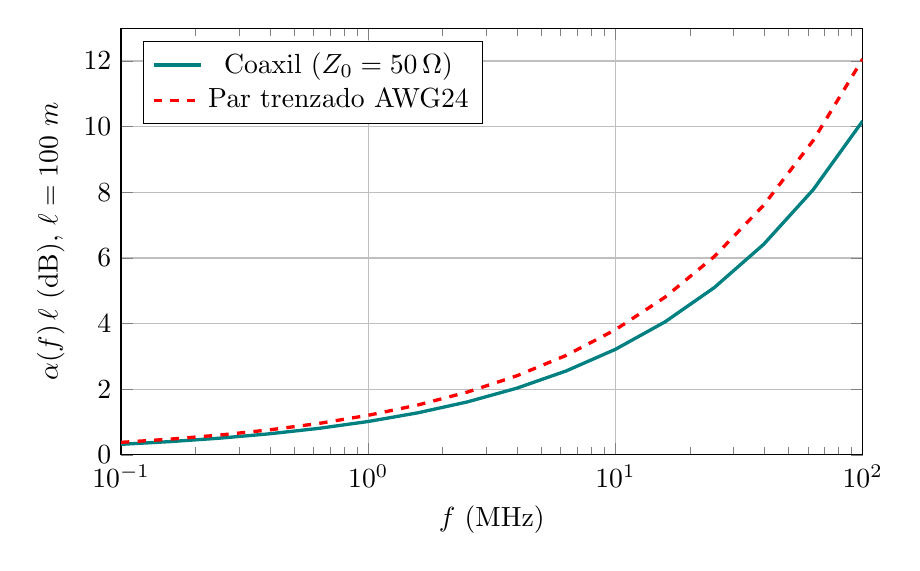
\begin{tikzpicture}
            \begin{axis}[
                width=11cm, height=7cm,
                xmode=log,
                xlabel={$f$ (MHz)},
                ylabel={$\alpha(f)\,\ell$ (dB), $\ell=100\ \text{m}$},
                xmin=0.1, xmax=100,
                ymin=0, ymax=13,
                legend pos=north west,
                grid=major,
                ]
                \addplot[teal, very thick, mark=none] coordinates {
                    (0.1000,0.3217) (0.1585,0.4049) (0.2512,0.5098) (0.3981,0.6418) (0.6310,0.8080) (1.0000,1.0172) (1.5849,1.2805) (2.5119,1.6121) (3.9811,2.0295) (6.3096,2.5550) (10.0000,3.2165) (15.8489,4.0494) (25.1189,5.0979) (39.8107,6.4179) (63.0957,8.0796) (100.0000,10.1716)
                };
                \addlegendentry{Coaxil ($Z_0=50\,\Omega$)}
                \addplot[Red, very thick, dashed, mark=none] coordinates {
                    (0.1000,0.3814) (0.1585,0.4801) (0.2512,0.6044) (0.3981,0.7609) (0.6310,0.9579) (1.0000,1.2060) (1.5849,1.5182) (2.5119,1.9113) (3.9811,2.4062) (6.3096,3.0292) (10.0000,3.8136) (15.8489,4.8010) (25.1189,6.0441) (39.8107,7.6091) (63.0957,9.5792) (100.0000,12.0595)
                };
                \addlegendentry{Par trenzado AWG24}
            \end{axis}
        \end{tikzpicture}
    \end{center}
    \caption{Atenuación $\alpha(f)\ell$ en función de la frecuencia, para $100\ \unit{\meter}$ de los dos cables del Ejemplo \ref{ejemplo:H canal}. La curva crece como $\sqrt f$ (efecto pelicular): es la versión física del bloque pasabajos $\hat H(f)$ de la Figura \ref{fig:distorsion canal}.}\label{fig:atenuacion comparada}
\end{figure}

\subsection*{Presupuesto de pérdidas}

Con $\alpha(f)$ en mano, podemos finalmente ponerle un número concreto a la atenuación $L$ que el Capítulo \ref{chapter:deteccion ruido} usó de forma genérica al analizar la cadena de repetidores (Ejemplos \ref{ejemplo:repeticion no regenerativa} y \ref{ejemplo:repetidor regenerativo}, Figura \ref{fig:repetidor regenerativo}): para un tramo de cable de longitud $\ell$, transmitiendo con velocidad de señalización $f_s$,
\begin{equation*}
    L\ (\text{en } \unit{\deci\bel}) = \alpha(f_s)\,\ell\cdot 8{,}686,
\end{equation*}
evaluando $\alpha$ (Ecuación \eqref{eq:alpha combinado}) a la frecuencia de señalización de interés. Este es, en definitiva, el \emph{presupuesto de pérdidas} (\emph{link budget}) del enlace guiado: dado un requerimiento de $S/N$ en recepción y la potencia de transmisión disponible, determina la máxima distancia entre repetidores (o entre transmisor y receptor, sin repetición).

\begin{ejemplo}[Espaciado de repetidores]
El Ejemplo \ref{ejemplo:repetidor regenerativo} del Capítulo \ref{chapter:deteccion ruido} suponía, sin justificarlo, una atenuación de $L=20\ \unit{\deci\bel}$ por etapa. Usando el cable coaxil del Ejemplo \ref{ejemplo:H canal} con una velocidad de señalización $f_s=10\ \unit{\mega\hertz}$ (donde, de la Figura \ref{fig:atenuacion comparada}, $\alpha(f_s)\ell$ vale $3{,}22\ \unit{\deci\bel}$ cada $100\ \unit{\meter}$), esos $20\ \unit{\deci\bel}$ se alcanzan a:
\begin{equation*}
    \ell = \frac{20\ \unit{\deci\bel}}{3{,}22\ \unit{\deci\bel}/100\ \unit{\meter}} \approx 620\ \unit{\meter}.
\end{equation*}
Es decir, para no exceder el presupuesto de pérdidas que aquel ejemplo asumía, un repetidor cada $620\ \unit{\meter}$ aproximadamente -- el número concreto que la Sección \ref{sec:dispersion pulsos} le debía al Capítulo \ref{chapter:deteccion ruido}.
\end{ejemplo}

Con esto entendimos, de punta a punta, de dónde sale $\hat H(f)$: de los parámetros $R,L,G,C$ (Sección \ref{sec:parametros distribuidos}), a través de la constante de propagación (Sección \ref{sec:ecuacion de onda}), hasta la atenuación creciente con la frecuencia que efectivamente limita el ancho de banda del canal (Sección \ref{sec:dispersion pulsos}). Queda una pregunta que la Sección \ref{sec:ecualizacion canal zfe} dejó pendiente al esbozar el filtro ecualizador sin resolverlo del todo: ahora que conocemos a $\hat H(f)$ con precisión, ¿podemos deshacer su efecto? Cerramos este capítulo respondiendo esa pregunta.

\section{Ecualización de canal}\label{sec:ecualizacion}

\subsection*{Resolución explícita del filtro de cero forzado}

Recordemos el planteo de la Sección \ref{sec:ecualizacion canal zfe} (Figura \ref{fig:filtro eq}): se recibe una onda con ISI, $x_R(t) = \sum_k a_k \tilde p(t-kT_s)$, y se la pasa por un filtro transversal de $2N+1$ ganancias $\{c_n\}_{n=-N}^N$, obteniendo una nueva onda PAM con pulso
\begin{equation*}
    \hat p(t) = \sum_{n=-N}^N c_n\, \tilde p(t-nT_s).
\end{equation*}
El criterio de \emph{cero forzado} (ZFE) pide $\hat p(kT_s)=0$ para $k=\pm 1,\ldots,\pm N$, junto con $\hat p(0)=1$ (para no perder la ganancia de la muestra útil). Escribamos esto explícitamente: evaluando $\hat p$ en $t=kT_s$,
\begin{equation*}
    \hat p(kT_s) = \sum_{n=-N}^N c_n\, \tilde p\big((k-n)T_s\big) = \sum_{n=-N}^N c_n\, \tilde p_{k-n},
\end{equation*}
donde abreviamos $\tilde p_m := \tilde p(mT_s)$ (las muestras del pulso recibido, el ``dato experimental'' que menciona la Sección \ref{sec:ecualizacion canal zfe}). La condición $\hat p(kT_s)=\delta_{k,0}$ para $k=-N,\ldots,N$ es entonces un sistema \emph{lineal} de $2N+1$ ecuaciones en las $2N+1$ incógnitas $c_n$:
\begin{equation}\label{eq:sistema zfe}
    \sum_{n=-N}^N \tilde p_{k-n}\, c_n = \delta_{k,0}, \qquad k=-N,\ldots,N.
\end{equation}
En forma matricial, $\mathbf P\,\mathbf c = \mathbf e_0$, donde $\mathbf c=(c_{-N},\ldots,c_N)^\top$, $\mathbf e_0$ es el vector con un $1$ en la posición central y ceros en el resto, y $\mathbf P$ es la matriz $(2N+1)\times(2N+1)$ de entradas $P_{k,n}=\tilde p_{k-n}$. Como $P_{k,n}$ depende solo de $k-n$, $\mathbf P$ es una \emph{matriz de Toeplitz} (constante en cada diagonal). La solución formal es $\mathbf c = \mathbf P^{-1}\mathbf e_0$, que existe siempre que $\mathbf P$ sea inversible -- lo es en la generalidad de los casos de interés práctico.

\begin{ejemplo}[ZFE de tres ganancias, $N=1$]\label{ejemplo:zfe n1}
Supongamos que, al medir el canal, obtenemos las muestras del pulso recibido (simétricas, un caso frecuente en la práctica): $\tilde p_0=1$, $\tilde p_{\pm 1}=0{,}2$, $\tilde p_{\pm 2}=0{,}05$ (y $\tilde p_m\approx 0$ para $|m|>2$). Con $N=1$, el sistema \eqref{eq:sistema zfe} tiene tres ecuaciones ($k=-1,0,1$) en las incógnitas $c_{-1},c_0,c_1$:
\begin{equation*}
    \begin{pmatrix} \tilde p_0 & \tilde p_{-1} & \tilde p_{-2} \\ \tilde p_1 & \tilde p_0 & \tilde p_{-1} \\ \tilde p_2 & \tilde p_1 & \tilde p_0 \end{pmatrix}
    \begin{pmatrix} c_{-1} \\ c_0 \\ c_1 \end{pmatrix}
    =
    \begin{pmatrix} 1 & 0{,}2 & 0{,}05 \\ 0{,}2 & 1 & 0{,}2 \\ 0{,}05 & 0{,}2 & 1 \end{pmatrix}
    \begin{pmatrix} c_{-1} \\ c_0 \\ c_1 \end{pmatrix}
    =
    \begin{pmatrix} 0 \\ 1 \\ 0 \end{pmatrix}.
\end{equation*}
Por la simetría de $\tilde p$, la solución también es simétrica, $c_{-1}=c_1$: de la primera ecuación, $c_{-1}(1{,}05) + 0{,}2\, c_0 = 0 \Rightarrow c_{-1}=-0{,}1905\, c_0$; sustituyendo en la segunda, $0{,}4\,c_{-1}+c_0=1 \Rightarrow 0{,}9238\, c_0 = 1$. Resolviendo:
\begin{equation*}
    c_0 \approx 1{,}0825, \qquad c_{-1}=c_1\approx -0{,}2062.
\end{equation*}
Verificando: $\hat p(0)=1$, $\hat p(\pm T_s)=0$ exactamente, como se pidió. Pero $\hat p(\pm 2T_s)\approx 0{,}0129$: \emph{no} es cero -- el ZFE con $N=1$ solo garantiza los ceros dentro del rango pedido, no más allá. Vamos a ver en breve, con precisión, por qué aparece este residuo y de qué depende.
\end{ejemplo}

Como ya anticipaba la Sección \ref{sec:ecualizacion canal zfe}, ajustar el filtro requiere conocer $\tilde p_m$, lo que se obtiene experimentalmente (transmitiendo un pulso o secuencia de entrenamiento conocida y midiendo la respuesta). En la práctica rara vez se calcula $\mathbf c=\mathbf P^{-1}\mathbf e_0$ de una sola vez: el canal puede variar levemente, o no conocerse con precisión de antemano, y es más robusto \emph{adaptar} los $c_n$ iterativamente a partir del error observado (algoritmos como LMS, \emph{Least Mean Squares}). No desarrollamos el algoritmo adaptativo en este curso -- el canal guiado es, a diferencia de uno inalámbrico, esencialmente \emph{invariante en el tiempo} una vez instalado, por lo que un ecualizador fijo, calibrado una vez, alcanza en la gran mayoría de los casos.

\subsection*{Equivalencia con la inversión del canal}

El residuo que quedó en el Ejemplo \ref{ejemplo:zfe n1} sugiere que el ZFE de $2N+1$ términos es una aproximación de algo más grande. Formalicémoslo. Para una sucesión genérica $\{x_n\}_{n\in\mathbb Z}$, definamos su \emph{transformada}
\begin{equation*}
    \hat X(f) := \sum_{n=-\infty}^{\infty} x_n\, \e^{-j2\pi f nT_s},
\end{equation*}
una función de $f$, periódica de período $f_s=1/T_s$ (los $x_n$ son, precisamente, sus coeficientes de Fourier). Aplicada a las muestras del pulso recibido, $\hat P_d(f):=\sum_m \tilde p_m\,\e^{-j2\pi fmT_s}$, es el análogo, en el dominio discreto de las muestras, del $\hat P(f)$ continuo que dedujimos en la Sección \ref{sec:dispersion pulsos}.

\begin{teorema}[ZFE de infinitos términos = inversión en frecuencia]\label{teorema:zfe inversion}
Si $\hat P_d(f)\neq 0$ para todo $f$, existe una única sucesión $\{c_n\}_{n\in\mathbb Z}$ que resuelve el sistema \eqref{eq:sistema zfe} \emph{sin truncar} ($k\in\mathbb Z$ en vez de $k=-N,\ldots,N$), y está dada por los coeficientes de Fourier de $1/\hat P_d(f)$:
\begin{equation*}
    c_n = f_s\int_{-f_s/2}^{f_s/2} \frac{\e^{j2\pi f nT_s}}{\hat P_d(f)}\; df.
\end{equation*}
\end{teorema}
\begin{proof}
Sea $\{c_n\}$ una solución del sistema sin truncar, y $y_k:=\sum_n \tilde p_{k-n}c_n$ (que por hipótesis vale $\delta_{k,0}$). Calculemos la transformada de $\{y_k\}$, sustituyendo $m:=k-n$:
\begin{equation*}
    \hat Y(f) = \sum_k y_k\, \e^{-j2\pi f kT_s} = \sum_n c_n \sum_m \tilde p_m\, \e^{-j2\pi f(m+n)T_s} = \left(\sum_n c_n\, \e^{-j2\pi fnT_s}\right)\left(\sum_m \tilde p_m\, \e^{-j2\pi fmT_s}\right) = \hat C(f)\,\hat P_d(f),
\end{equation*}
el \emph{teorema de convolución} discreto -- exactamente análogo al continuo ya conocido: la transformada de una convolución es el producto de las transformadas. Por otro lado, $y_k=\delta_{k,0}$ para todo $k$ da $\hat Y(f)=\sum_k \delta_{k,0}\e^{-j2\pi fkT_s}=1$. Combinando ambas expresiones para $\hat Y(f)$:
\begin{equation*}
    \hat C(f)\, \hat P_d(f) = 1 \quad\Longrightarrow\quad \hat C(f) = \frac{1}{\hat P_d(f)},
\end{equation*}
bien definida en todo $f$ porque $\hat P_d(f)\neq 0$ por hipótesis. Como $\{c_n\}$ son, por construcción, los coeficientes de Fourier de $\hat C(f)$, la fórmula de inversión de Fourier los determina de manera única.
\end{proof}

Esto es exacto, no una analogía: el ZFE de infinitos coeficientes \emph{es}, literalmente, la inversión de $\hat P_d(f)$ -- el mismo cociente ideal que uno esperaría escribir directamente en frecuencia, ahora obtenido a partir del sistema de ecuaciones que ya conocíamos, sin agregar ninguna herramienta nueva más que la transformada de una sucesión. El filtro finito de $2N+1$ términos del Ejemplo \ref{ejemplo:zfe n1} es, entonces, precisamente lo que sugiere su nombre: los $2N+1$ coeficientes centrales de esta serie de Fourier infinita, truncada -- y el residuo $\hat p(\pm 2T_s)\approx 0{,}0129$ que encontramos ahí es, ni más ni menos, el error de truncar una serie de Fourier a pocos términos.

\begin{remark}[Verificación en el caso trivial]
Si el pulso recibido ya es de Nyquist ($\tilde p_m=\delta_{m,0}$, sin ISI), entonces $\hat P_d(f)\equiv 1$ y el Teorema \ref{teorema:zfe inversion} da $c_0=1$, $c_n=0$ para $n\neq 0$: el ecualizador resulta el filtro identidad. No hay nada que corregir, como debe ser.
\end{remark}

\subsection*{El costo de invertir en banda ancha}

La simplicidad de $\hat C(f)=1/\hat P_d(f)$ esconde un problema serio, que ya el texto original de la Sección \ref{sec:ecualizacion canal zfe} anticipaba cualitativamente (``si algunas ganancias son muy altas, el ruido puede verse amplificado''): en cualquier frecuencia donde $\hat P_d(f)$ sea chico, el ecualizador necesita una ganancia $|\hat C(f)|=1/|\hat P_d(f)|$ enorme. Y $\hat P_d(f)$ hereda, en cada punto, la forma de $\hat H(f)$ que dedujimos en la Sección \ref{sec:dispersion pulsos} (Figura \ref{fig:atenuacion comparada}): decrece con la frecuencia, así que corregirlo cerca del borde de la banda pedida exige ganancias cada vez mayores. El problema es que el ruido a la entrada del ecualizador (Capítulo \ref{chapter:deteccion ruido}) tiene energía en todas las frecuencias, y esa misma ganancia enorme amplifica el ruido en esa banda exactamente tanto como reconstruye la señal. En el límite, si $\hat P_d(f)\to 0$ en alguna banda (un cero real del canal, no solo una atenuación fuerte), $\hat C(f)\to\infty$ ahí: el ZFE intenta reconstruir información que, en esa banda, ya se perdió irremediablemente en ruido.

Esto sugiere una idea distinta, que retomamos con toda su fuerza en el Capítulo \ref{chapter:ofdm}: en vez de invertir $\hat P_d(f)$ de una sola vez sobre todo el ancho de banda, \emph{partir} la banda en tramos angostos, cada uno lo suficientemente chico como para que $\hat P_d(f)$ sea aproximadamente \emph{plano} dentro de él. En cada tramo, invertir $\hat P_d(f)$ ya no requiere una ganancia extrema -- es, esencialmente, dividir por una constante (un único número complejo por tramo) en vez de por una función que varía mucho. La idea completa -- banda ancha partida en muchos subcanales angostos, cada uno ecualizado trivialmente -- es exactamente lo que hace OFDM, y es el motivo por el cual, adelantándolo aquí, ese capítulo empieza a tener sentido: \textbf{OFDM es, en el fondo, una forma práctica de resolver el problema de ecualización que acabamos de plantear}, evitando el costo de invertir en banda ancha.

Con esto se cierra el círculo completo de este capítulo: de los parámetros físicos de la línea llegamos a $\hat H(f)$, entendimos por qué distorsiona la señal, y mostramos cómo deshacer exactamente esa distorsión -- incluso cuantificando el costo de hacerlo en banda ancha, la motivación última de OFDM. En el próximo capítulo atacamos el segundo problema que todo sistema de comunicaciones real debe resolver y que hasta ahora dimos por sentado: el sincronismo entre transmisor y receptor.






